\begin{frame}
\frametitle{Суперблок}
\begin{itemize}
  \item ФС начинается с суперблока
  \begin{itemize}
    \item суперблок - это структура, которая хранит общую информацию о ФС
    \begin{itemize}
      \item магическое число/строка - чтобы убедиться, что на диске хранится
      именно наша ФС;
      \item размер блока ФС;
      \item версия ФС;
      \item ссылки на какие-то общие структуры ФС, например, список свободных
      блоков.
    \end{itemize}
    \item Суперблок хранится в каком-то известном месте диска
    \begin{itemize}
      \item иногда на диске хранится несколько копий супеблока, чтобы если один
      из них испортится, то можно будет использовать другой;
      \item потеря суперблока, это практически потеря ФС.
    \end{itemize}
  \end{itemize}
\end{itemize}
\end{frame}

\begin{frame}
\frametitle{Индексные узлы (Inode-ы)}
\begin{itemize}
  \item Inode - важная структура в классических Unix-овых (и не только) ФС
  \begin{itemize}
    \item Inode пресдтавляет сущность внутри ФС (файл/каталог):
    \begin{itemize}
      \item хранит права/привелегии доступа, даты модификации и прочее;
      \item размер файла/каталога и \emph{раcположение его блоков на диске};
      \item примерное представление об содержимом Inode вам может дать
      \emph{man 2 stat};
    \end{itemize}
    \item каждый Inode имеет уникальный идентификатор, по которому его можно
    найти на диске
    \begin{itemize}
      \item зная идентификатор вы можете легко найти Inode на диске;
      \item в классических ФС, при форматировании выделяется таблица Inode-ов;
      \item идентификатор Inode - это просто его позиция в таблице.
    \end{itemize}
  \end{itemize}
\end{itemize}
\end{frame}

\begin{frame}
\frametitle{Описание расположения блоков}
\begin{center}
  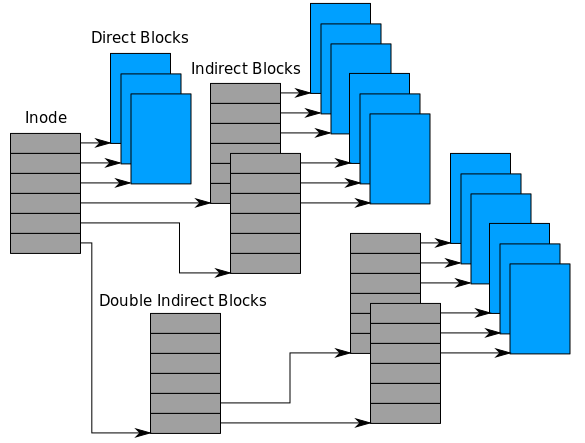
\includegraphics[width=.8\linewidth]{inode.png}
\end{center}
\end{frame}

\begin{frame}
\frametitle{Fast File System}
\begin{itemize}
  \item Fast File System - первая из классических Unix-овых ФС, в которой были
  учтены особенности диска
  \begin{itemize}
    \item не то, чтобы до этого никто не заботился о производительности;
    \item но ребята из Berkely, которые создали FFS довольно буедительно
    показали, что диск в ФС того времени использовался неэффективно.
  \end{itemize}
  \item В Fast File System минимальный размер блока - 4Kb
  \begin{itemize}
    \item т. е. за одно обращение к диску ФС пишет/читаете сразу 8 секторов;
    \item это привело к заметному увеличению скорости работы ФС, что ясно
    показало, что другими ФС диск использовался не эффективно.
  \end{itemize}
\end{itemize}
\end{frame}

\begin{frame}
\frametitle{Цилиндровые группы}
\begin{itemize}
  \item Цилиндровая группа - группа блоков, которые расположены на диске рядом
  \begin{itemize}
    \item цилиндровые группы - еще одна оптимизация введенная в FFS;
    \item каждая цилиндровая группа содержит свой набор Inode-ов, битовую карту
    свободных/занятых блоков внутри группы и прочее.
  \end{itemize}
  \item Цилиндровые группы используются для более эффективной аллокации ресурсов
  на диске:
  \begin{itemize}
    \item достаточно большие куски файла пытаются положить в одну цилиндровую
    группу;
    \item Inode-ы файлов в одном каталоге, стараются также положить в одну
    цилиндровую группу;
    \item при этом стараемся не заполнять цилинддровые группы под завязку.
  \end{itemize}
\end{itemize}
\end{frame}

\begin{frame}
\frametitle{Классические Unix-овые ФС}
\begin{itemize}
  \item FFS - это предшественник классических Unix-овых ФС
  \begin{itemize}
    \item сейчас никто не использует FFS (скорее всего), но многие пользуются
    ее наследниками: ext3 и ext4 (ext2, если кто-то ей пользуется).
  \end{itemize}
  \item Многие детали отличаются, но многие идеи остаются:
  \begin{itemize}
    \item например, каталог это не просто набор записей, а HTree/B+-tree или
    какая-то подобная индексная структура данных;
    \item журналирование для обеспечения консистентности вместо soft updates;
    \item а цилиндровые группы остались, хотя возможно называются по-другому.
  \end{itemize}
\end{itemize}
\end{frame}
